\documentclass[12pt]{report}
\usepackage{polski}
\usepackage[utf8]{inputenc}
\usepackage{graphicx}
\graphicspath{ {../} }
\begin{document}

\author{Jakub Ogrodowczyk}
\section*{Wnioski}

Jak widać na poniższych wykresach, wraz z ilością generowanych punktów
rośnie dokładność naszego przybliżenia. W szczególności dla niewielkich wartości
n, wyniki dla poszczególnych powtórzeń znacznie odbiegają od faktycznego wyniku.

\begin{figure}[h]
\centering
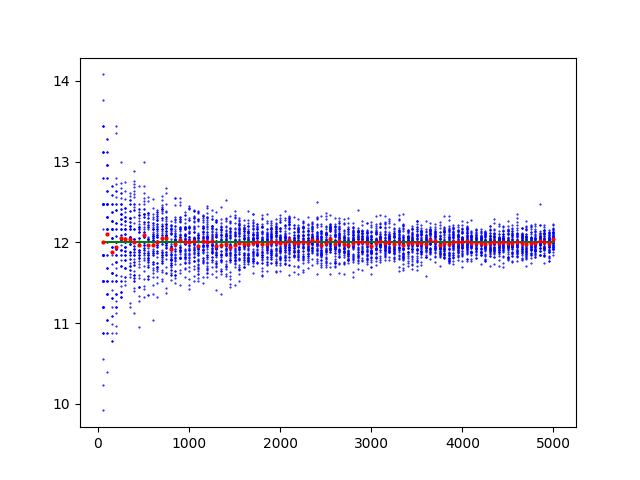
\includegraphics{sqrt3x.png}
\caption[Example .]{Wykres dla \(\int_{0}^{8} \sqrt[3]{x} \,dx\)}
\label{...}
\end{figure}

\begin{figure}[h]
\centering
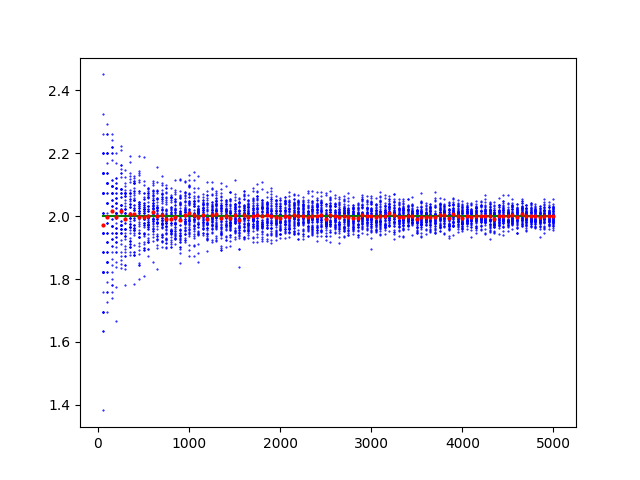
\includegraphics{sinx.png}
\caption[Example .]{Wykres dla \(\int_{0}^{\pi} sin(x) \,dx\)}
\label{...}
\end{figure}
    
\begin{figure}[h]
\centering
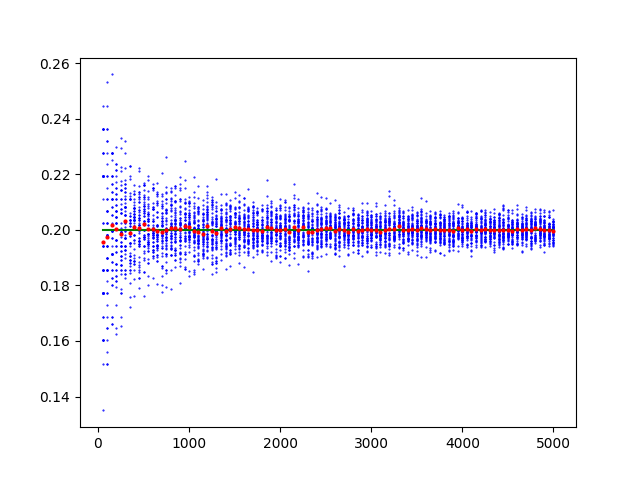
\includegraphics{4x(1-x)3.png}
\caption[Example .]{Wykres dla \(\int_{0}^{1} 4x(1-x)^{3} ,dx\)}
\label{...}
\end{figure}

\end{document}